\section{Ingestion-Pipeline (Datenverarbeitung)}
Damit Dokumente durchsuchbar werden, müssen sie eine komplexe Verarbeitungspipeline durchlaufen. Dieser Prozess wird vom \texttt{IndexingService} gesteuert und ist rechenintensiv.

\begin{figure}[H]
    \centering
    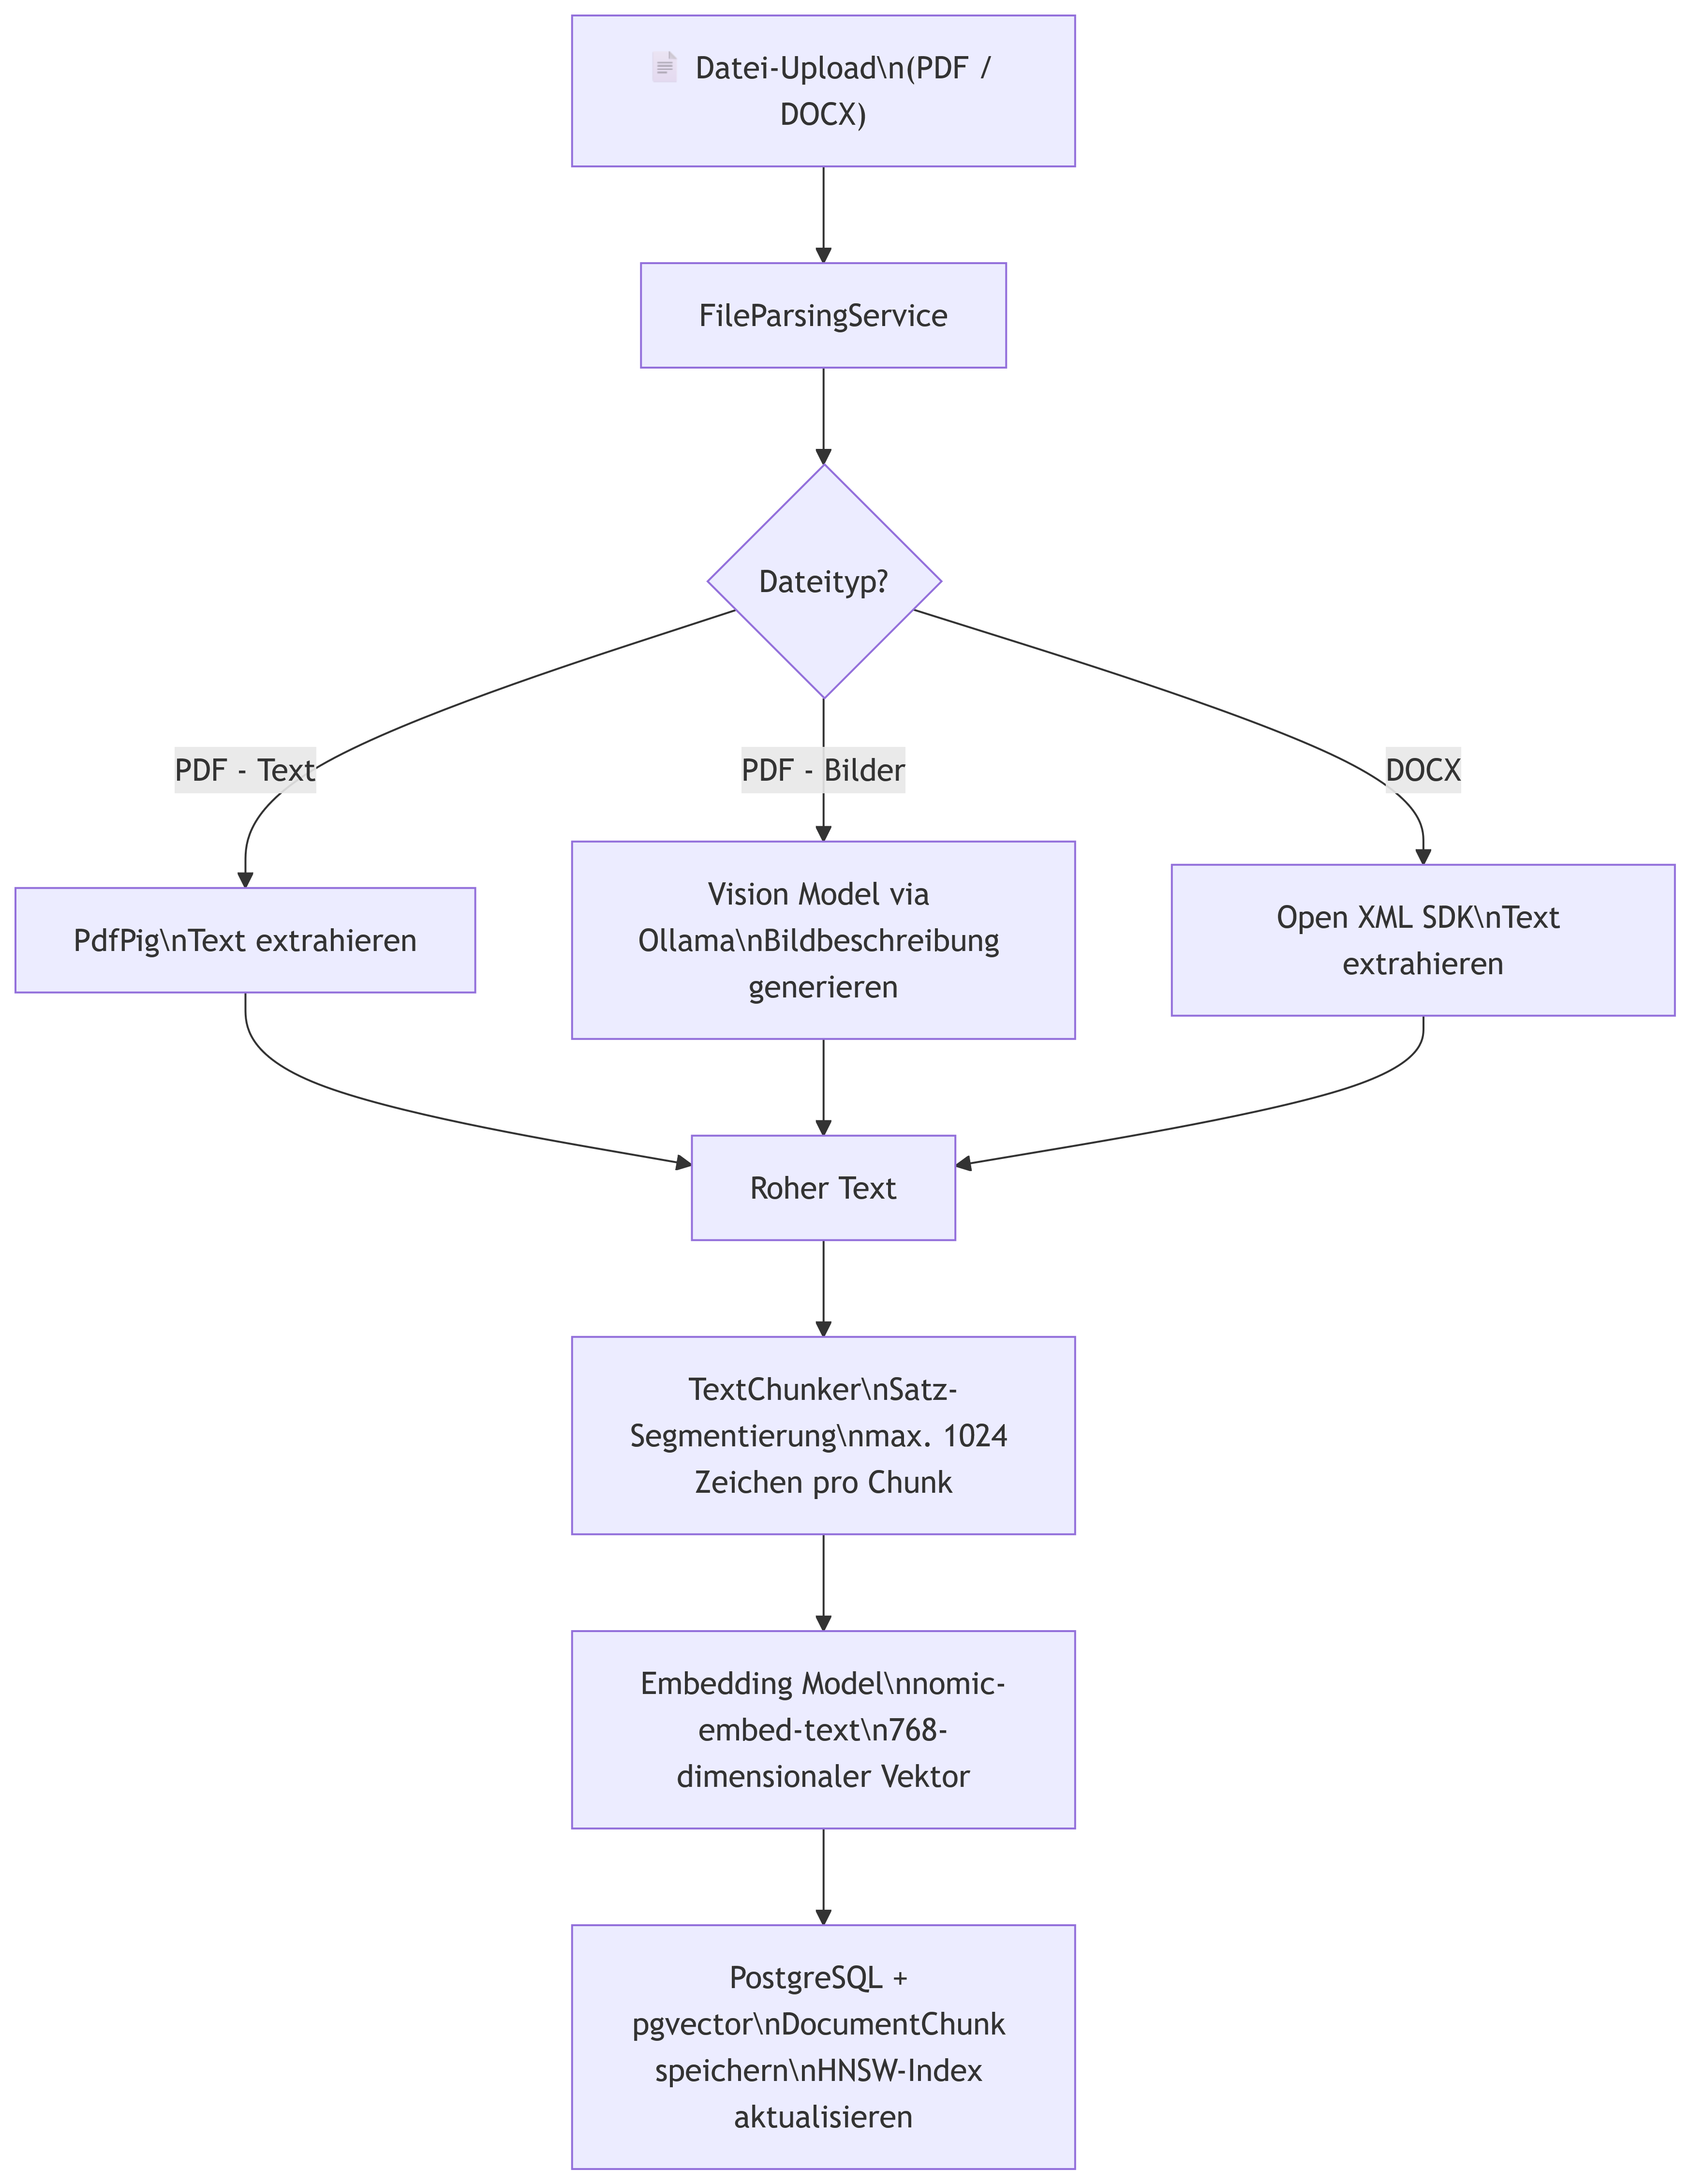
\includegraphics[width=0.85\textwidth]{img/ingestion_pipeline.png}
    \caption{Ablaufdiagramm der Ingestion-Pipeline in EduShelf}
    \label{fig:ingestion_pipeline}
\end{figure}

\subsection{1. Textextraktion (OCR \& Parsing)}
Der \texttt{FileParsingService} analysiert den Dateityp und wählt die passende Strategie:
\begin{itemize}
    \item \textbf{PDF-Verarbeitung mit PdfPig:} Für PDF-Dateien wird die Bibliothek \textit{UglyToad.PdfPig} verwendet. Sie erlaubt den Zugriff auf den rohen Textstream sowie die Extraktion von Bildern.
    \item \textbf{Hybride Bildanalyse:} Eingebettete Bilder werden isoliert und an ein lokales Vision-Model (via Ollama) gesendet. Der Prompt "Describe this image in detail" generiert eine textuelle Beschreibung, die in den Dokumentenindex einfließt. Dies ermöglicht die semantische Suche nach Bildinhalten (z.B. Diagramme, Graphen).
    \item \textbf{DOCX:} Nutzung des Open XML SDKs zum strukturierten Auslesen des \texttt{MainDocumentPart}.
\end{itemize}

\subsection{2. Chunking (Intelligente Segmentierung)}
LLMs haben ein begrenztes Kontextfenster, und die semantische Suche verliert bei zu großen Textblöcken an Präzision. Der \texttt{TextChunker} implementiert daher eine mehrstufige Strategie:
\begin{enumerate}
    \item \textbf{Satz-Tokenisierung:} Der Text wird zunächst anhand von Satzzeichen (. ! ?) in einzelne Sätze zerlegt.
    \item \textbf{Rekombination:} Diese Sätze werden iterativ zu einem Chunk zusammengefügt, bis eine konfigurierte Grenze von ca. 1024 Zeichen erreicht ist. Dies stellt sicher, dass semantische Zusammenhänge (Sätze) nicht willkürlich in der Mitte durchschnitten werden.
    \item \textbf{Token-Limit:} Zusätzlich wird sichergestellt, dass die Chunks eine maximale Token-Anzahl (für das Embedding-Model) nicht überschreiten.
\end{enumerate}

\begin{lstlisting}[language={[Sharp]C}, caption={Implementierung der Satz-Segmentierung in TextChunker.cs}]
public static List<string> SplitBySentence(string text)
{
    // Nutzung von Regex Lookbehind (?<=...), um das Satzzeichen zu behalten
    var sentences = Regex.Split(text, @"(?<=[\.!\?])\s+");
    return new List<string>(sentences);
}
\end{lstlisting}
Das simple Splitten nach Zeichenanzahl würde Sätze zerreißen und den Kontext zerstören. Der hier gezeigte Ansatz garantiert semantische Integrität.

\subsection{3. Embedding und Vektorspeicherung}
Jeder Text-Chunk wird in einen hochdimensionalen Vektor umgewandelt und effizient gespeichert.
\begin{itemize}
    \item \textbf{Embedding-Modell:} Nutzung von state-of-the-art Modellen wie \textit{nomic-embed-text}, die semantische Ähnlichkeiten im Vektorraum abbilden.
    \item \textbf{HNSW Index:} In der PostgreSQL-Datenbank wird für die Spalte \texttt{Embedding} ein HNSW (Hierarchical Navigable Small World) Index angelegt.
    \begin{verbatim}
modelBuilder.Entity<DocumentChunk>()
    .HasIndex(dc => dc.Embedding)
    .HasMethod("hnsw")
    .HasOperators("vector_l2_ops");
    \end{verbatim}
    Dieser Index ermöglicht eine extrem schnelle Nearest-Neighbor-Suche (ANN) auch bei Millionen von Vektoren, da nicht die gesamte Tabelle gescannt werden muss.
\end{itemize}
